\subsection{Yolo Function}

The YOLOv8 model has proven its efficacy in detecting individuals within the camera frame, significantly contributing to the overall safety and situational awareness of the autonomous drone.

\begin{figure}[H]
    \centerline{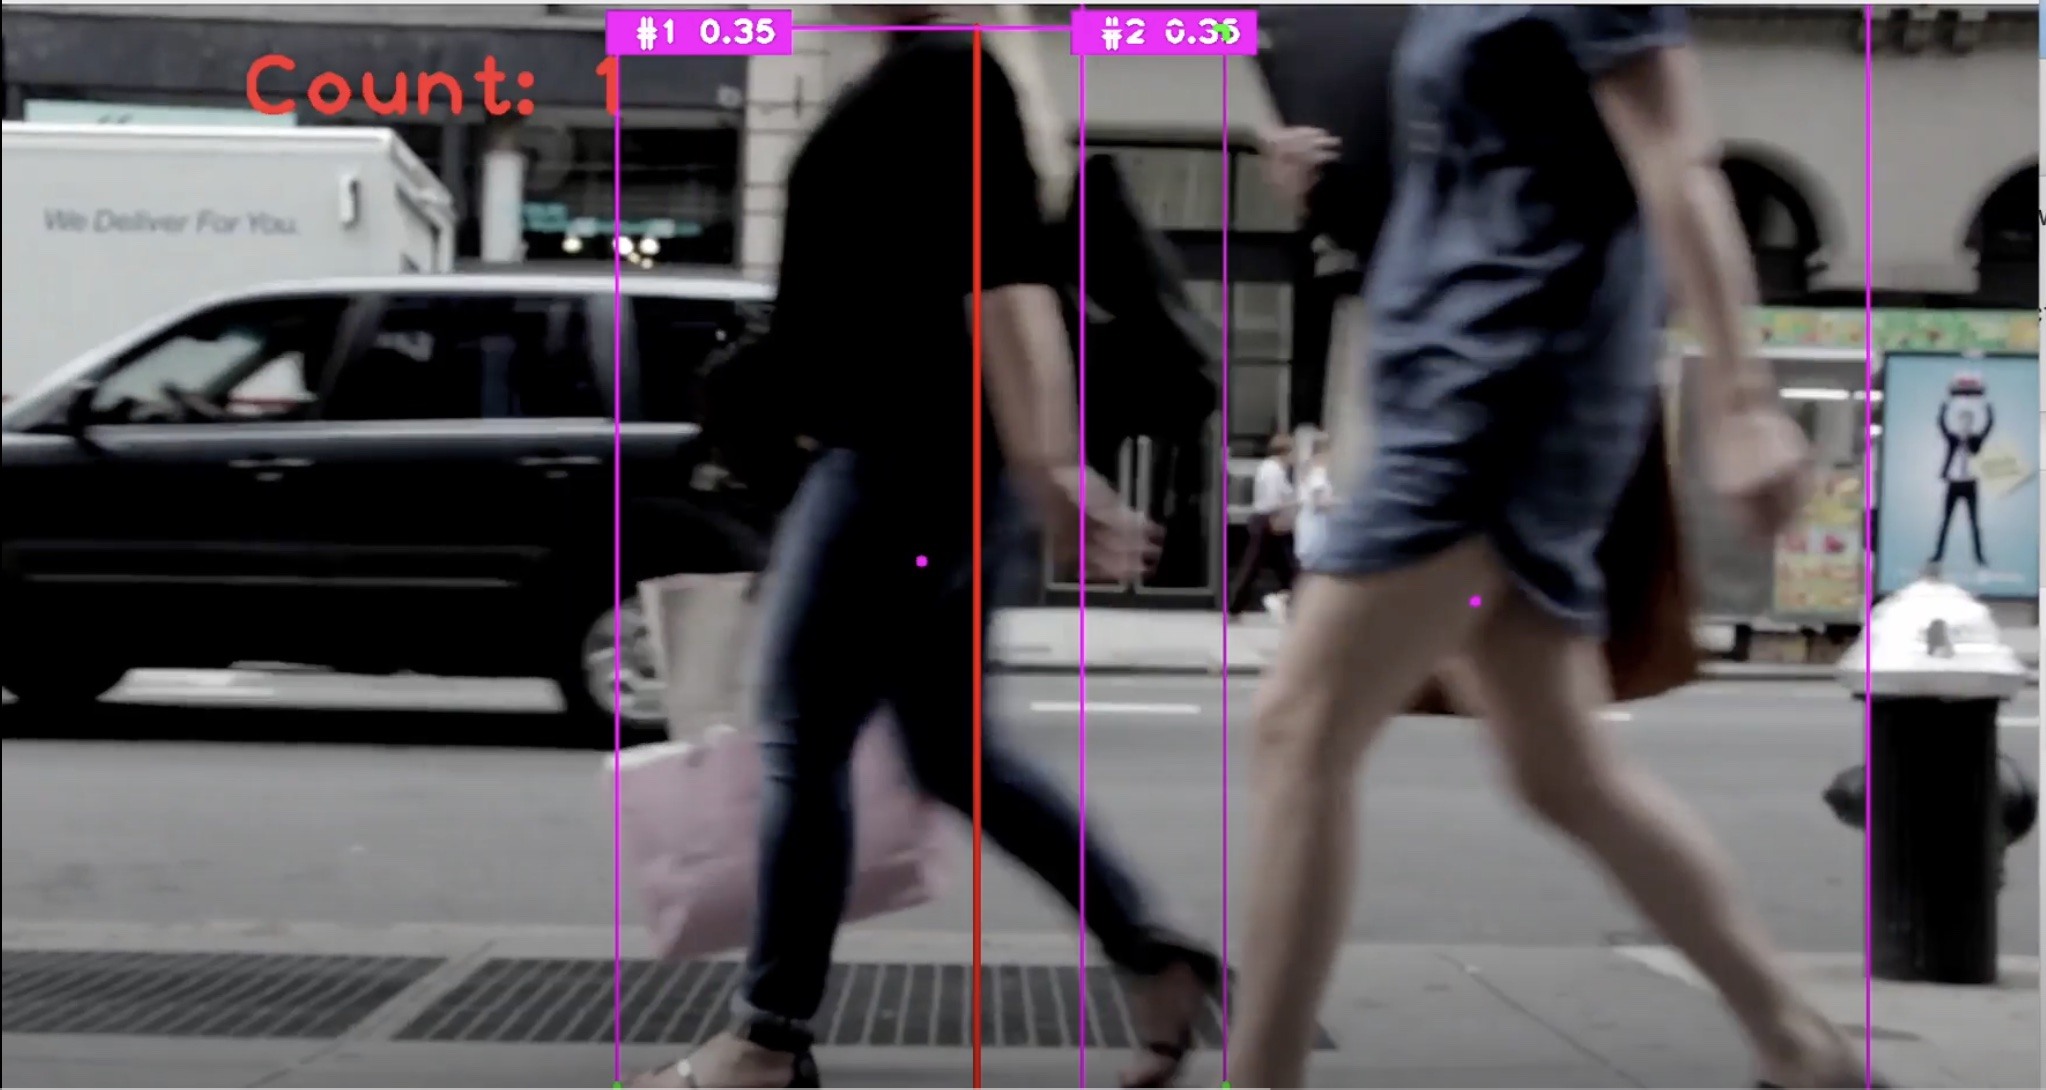
\includegraphics[width=0.5\textwidth]{Figures/Results/people counting.jpg}}
    \caption{People Detection and Counting.}
    \label{fig3c1}
\end{figure}

\begin{figure}[H]
    \centerline{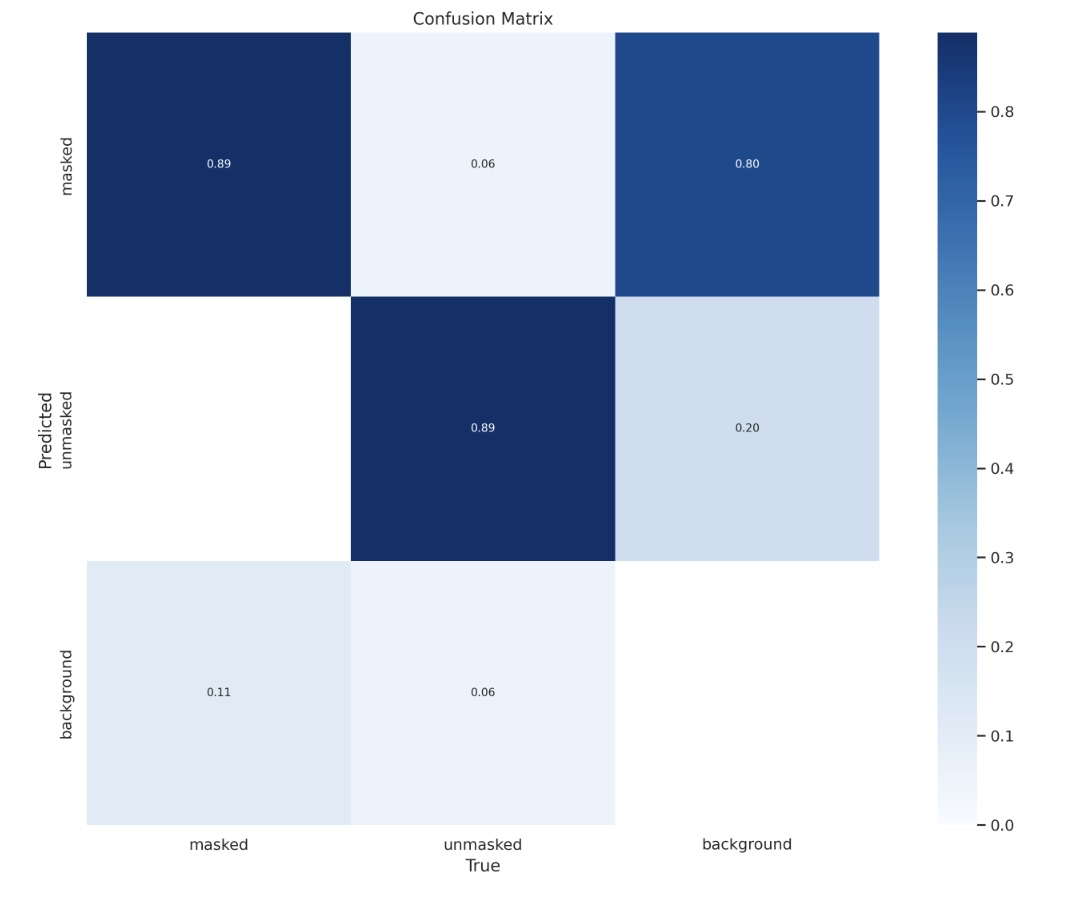
\includegraphics[width=0.5\textwidth]{Figures/Results/Confusion Matrix.jpg}}
    \caption{Confusion Matrix of Mask Detection Model.}
    \label{fig3c2}
\end{figure}

Fig.~\ref{fig3c1} shows the outcomes of the people counting function. Initially, individuals in each frame are identified by a red bounding box. YOLOv8 tracks these individuals and tallies them when the center of the bounding box intersects with a predefined line. For this specific experiment, the line is positioned at the center of the image.

Fig.~\ref{fig3c2} illustrates the performance metrics of the mask detection model. The achieved accuracy of this model is 89{\%}, indicating that individuals wearing masks can be correctly identified with an accuracy rate of 89{\%}.